\section{Preparing VASP-files before starting ENVISIoN}
Before visualizations can be made of input data from VASP, the user have to make sure that VASP-files are made in correct format. This applies to a couple main files in VASP that the user has specified before their VASP-run and also after their VASP-run. The restrictions on the formating of VASP-files are a byproduct of the fact that ENVISIoN has a couple limitations in it's parsing of VASP-files. These limitations are by no way intentional and they are born from theoretical sources and from the time-restrictive nature of the project development itself. 
\subsection{Preparing for bandstructure visualization}

Before deciding to do any visualization of bandstructures at all, be sure that the VASP-files OUTCAR and KPOINTS are available in the VASP-directory you wish to visualize from. Bandstructure visualization can only be made for eight types of brillouin zones if the user wishes to do so. Namely the following: Primitive Cubic (CUB), Body-Centered Cubic (BCC), Face-Centered Cubic (FCC), Primitive Tetragonal (TET), Primitive Hexagonal (HEX), Primitive Orthorhombic (ORC), Primitive Triclinic type 1a/2a (TRI1a/TRI2a) and Primitive Triclinic type 1b/2b (TRI1b/TRI2b). These brillouin zones have fixed symmetry k-points and are specified in an article by Wahyu Setyawan and Stefano Curtarolo \cite{k-points}.

If the user wish to visualize the bandstructure of any other type of brillouin zone, the parser for bandstructures will be unable to interpret the data from VASP. 

Another requirement for a successful visualization of the bandstructure of a brillouin zone type is to format the KPOINTS-file in a specific way such as is illustrated in figure \ref{fig:VASP_band} below. Observe how every two coordinates represents a line between two high-symmetry points as chosen by the $"$line$"$ in the third row, and how each of these pair of coordinates are separated by a blank row for aesthetical reasons. The parser can only handle reciprocal high-symmetry points so make sure that the fourth line in the KPOINTS-file has the word $"$reciprocal$"$ written with no indentation, as shown in the figure.

\begin{figure}[H]
    \centering
    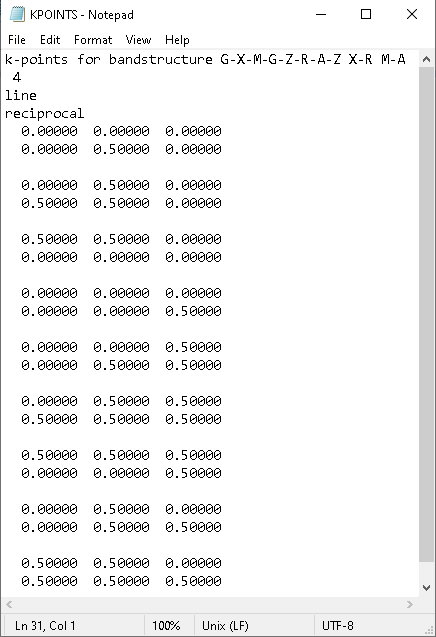
\includegraphics[scale = 0.53]{Images/usermanual_band_TET.png}
    \caption{KPOINTS-file for bandstructure calculation of a TET brillouin zone.}
    \label{fig:VASP_band}
\end{figure}

\subsection{Preparing for fermi-surface visualization}

Make sure that a KPOINTS-file and a EIGENVAL-file is present in the VASP-directory you want to input in ENVISIoN. 

When choosing to visualize fermi-surfaces, make sure that you use the format shown in figure \ref{fig:VASP_fermisurface} for the KPOINTS-file. During visualization of the fermi-surface of a crystal, we want a very big mesh of k-points and an optimal mesh is 10x10x10. Hence make sure that you the fourth row in KPOINTS is at least 10 on each position, as shown in the figure. A very important thing to also note is that the user has to supply the second row with only the a zero, as shown in the figure, as it will force VASP to generate a mesh in the size specified on the fourth row of the file during a VASP-run.

\begin{figure}[H]
    \centering
    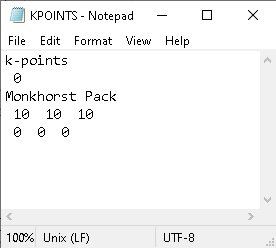
\includegraphics[scale = 0.55]{Images/usermanual_fermisurface.png}
    \caption{KPOINTS-file for fermi-surface visualization.}
    \label{fig:VASP_fermisurface}
\end{figure}

Another, very important, thing to note is that the fermi-surface visualization requires the flag ISYM in the INCAR-file of VASP to be set to the value -1 before a VASP-run. If ISYM is not set to -1, the parser for Fermi-surface will not be able to extrapolate the k-points that are given by VASP, since they are symmetric. If you strive to improve your visualization of the fermi-surface of a crystal, simply increase each integer on the fourth row on the figure above from 10 and above. Observe that the fifth row must have zeroes in order to generate a mesh centered in a origin of the Monkhorst-Pack, without any shifts from this origin. This is for the sake of avoiding errors in the VASP-run.

\subsection{Preparing for unitcell visualization}
\label{section_unit}

Make sure that the VASP-files POTCAR and POSCAR are available in your VASP-directory before you decide to visualize the unitcell. 

For the unitcell visualization, it is very important how you have written the POTCAR-file in relation to the POSCAR-file. Say you have a crystal structure made of three atomic species and you want to do a VASP-run of it. You will first have to find the POTCAR-files for each atomic species, which is supplied by VASP itself. Then you concat them in order to create a single POTCAR-file which represent all atomic species in a single file. Now the dangerous and very common mistake to do in this case is that you concat the separate atomic species POTCARs in an order that does not consist with the order written in the POSCAR-file. This can lead to wrong conclusions of your VASP-calculations. Figure \ref{fig:VASP_unit} examplifies the correct way of concatting POTCARs.

\begin{figure}[H]
    \centering
    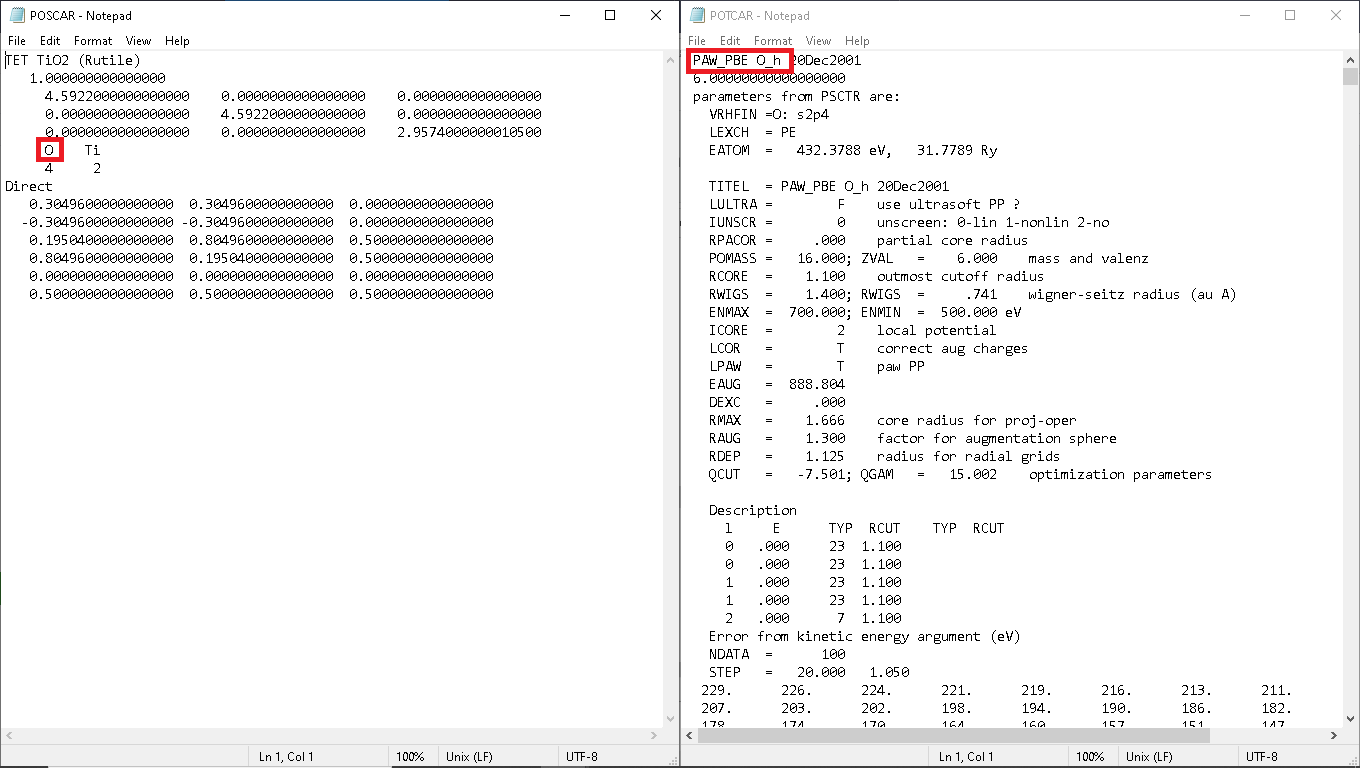
\includegraphics[scale = 0.48]{Images/usermanual_unit_TET.png}
    \caption{In this example with the crystal TiO2, the POSCAR-file has Oxygen written as the first atomic species (red box) and hence the common POTCAR has the pseudopotentials of Oxygen atoms concat first and the pseudopotentials of titanium atoms second.}
    \label{fig:VASP_unit}
\end{figure}

To successfully visualize the unitcell, the user has to make sure that there is no indentation in the row where the user specifies if the atomic positions are given in direct or cartesian coordinates in the POSCAR-file. There is also a requirement that all values in the POSCAR-file, besides the row which supplies the number of atoms per atomic species (which are given in integer form), are given in decimal form (float form). Figure \ref{fig:VASP_unit_1} below shows the correct format of POSCAR in the example with Rutile. Notice how the order of the atomic positions are consistent with the order of the atomic species, which is emphasized by the red box for the O-atom positions and the blue box for the Ti-atom positions.

\begin{figure}[H]
    \centering
    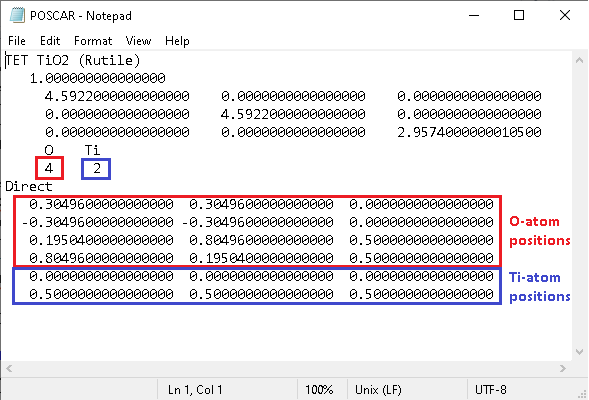
\includegraphics[scale = 0.50]{Images/usermanual_unit_TET_2.png}
    \caption{Example of the correct format of POSCAR-file with the crystal TiO2.}
    \label{fig:VASP_unit_1}
\end{figure}

\subsection{Preparing for DOS visualization}

Make sure that the VASP-files POTCAR, POSCAR, INCAR and DOSCAR are available in your VASP-directory before you decide to visualize the density of states. \\

To ensure an error-free visualization of DOS, follow the directions mentioned in the section \emph{\nameref{section_unit}}, since unitcell data is acquired simultaneously with DOS data with the VASP parser for DOS visualization.

\subsection{Preparing for electron density visualization}

Make sure that the VASP-files POTCAR, POSCAR and CHG are available in your VASP-directory before you decide to visualize the electron density. In the VASP-file INCAR, make sure that LCHARG flag is not set to False, in order to force VASP to write into the CHG-file during the VASP-run. Also make sure that ISYM flag in the VASP-file INCAR is not set to -1 before a VASP-run, which is done for the fermi-surface visualization, as this can cause a wrong visualization of the electron density.\\

To ensure an error-free visualization of electron density, follow the directions mentioned in the section \emph{\nameref{section_unit}}, since unitcell data is acquired simultaneously with electron density data with the VASP parser for electron density visualization.

\subsection{Preparing for force visualization}
Make sure the VASP-files POSCAR and OUTCAR are available in your VASP-directory before visualising force vectors. If these two files are present and in unchanged condition the force vector visualisation should commence non-erroneously.

Notice that in many VASP-directories the forces acting on atoms will be zero, in these cases the vectors will instead be represented as discs in the middle of the atoms, analogous to having a length of zero.

\subsection{Preparing for molecular dynamics visualization}
Make sure that the VASP-files POSCAR, OUTCAR and XDATCAR are available in your VASP-directory before you decide to visualize the molecular dynamics. The IBRION flag has to be set to 0 in the VASP-file OUTCAR for the visualization to run, it's the IBRION flag that decides if  molecular dynamics is possible or not. The NSW flag in the OUTCAR file will be the amount of time steps for the visualization, check if this seems to be correct. \\

The XDATCAR file should contain data for the positions of each atom for all the time steps, if something is wrong with the XDATCAR file the IBRION flag in the OUTCAR flag probably is not set to the correct value for molecular dynamics. From the POSCAR file you will receive data about the elements and the amount of each sort of atom.   

\newpage

\section{Preparing ELK-files before starting ENVISIoN}
Before visualizations can be made of input data from ELK, the user have to make sure that the correct ELK-files are provided and made in the correct format for the visualization that the user wants to run.

\subsection{Preparing for unitcell visualization}

Make sure that the ELK-files INFO.OUT and EQATOMS.OUT are available in your ELK-directory before you decide to visualize the unitcell. If thees two files exist the visualization should be able to run.  

\subsection{Preparing for force visualization}

To run a force visualization task nr 2 must be run when elk performs calculations. Look in the elk.in and confirm that this is done. Make sure the ELK-files INFO.OUT and EQATOMS.OUT are available in your ELK-directory before visualising force vectors. If these two files are present in unchanged condition and task nr 2 has bean preformed the force vector visualisation should commence non-erroneously. If the forces acting on atoms is zero the vectors will instead be represented as discs in the middle of the atoms, analogous to having a length of zero. 

\subsection{Preparing for elf visualization}
To run a elf visualization task nr 53 must be run when elk performs calculations. Look in the elk.in and confirm that this is done. Make sure the ELK-files INFO.OUT and ELF3D.OUT are available in your ELK-directory before visualising elf. If these two files are present in unchanged condition and task nr 53 has bean preformed the elf visualisation should commence non-erroneously.



\newpage

